\documentclass{jsarticle}
\usepackage[dvipdfmx]{graphicx}
\usepackage{subcaption}
\captionsetup[figure]{justification=centering}
\captionsetup[table]{justification=centering}
\usepackage[ipa]{pxchfon}

\begin{document}
\title{{\vspace*{-30mm}}{\huge 研究計画書}}
\author{\large 千葉工業大学 先進工学部 未来ロボティクス学科 \vspace*{2mm}\\20C1015 今井悠月}
\date{}
\maketitle




\section{研究題目}
視覚と行動の end-to-end 学習により経路追従行動を模倣する手法の提案\\
\hspace{6.25zw}(動的環境による影響を緩和させる手法の提案)

\section{背景・目的}
本研究グループでは, 移動ロボットにおける地図ベースの経路追従行動を, 視覚を入力とする行動に, 模倣する手法を提案し, 
その有効性を実験により検証してきた[1][2]. 地図ベースの経路追従とは, 予め作成した地図とLiDARなどのセンサを用いて, 
自己位置推定, 経路計画, 制御などの複数のタスクを実行することで, 経路を追従させる方法である[3]. 
本研究グループが提案する手法(図1)を用いることで, 地図ベースの経路追従とカメラ画像を入力とする
経路追従の2つのナビゲーション手段を得られる. 
この2つの手段を状況に応じて高い信頼性が見込まれる方を選択することで, 経路追従を継続できる可能性が高まる.
地図ベースの経路追従行動の模倣には, 入出力関係を直接学習する end-to-end 学習器を用いる.\\\hspace{1zw}
近年, end-to-end 学習による自律移動手法がいくつか研究されている.
例えば, Muller らは, 人が操作したコントローラ操作を教師データとして学習することで, 
オフロード環境で障害物を回避しながら走行できることを確認した[4].
また, Bojarski らは画像と人が操作した制御コマンドを end-to-end 学習するこ
とで, 自動車を対象とした自律移動手法を提案した[5].
しかし, それらの研究では必ずしも学習した経路を追従できる
わけではなく, コースの一部で経路追従に失敗する様子が確認されている.
その一因として, 動的環境の影響により, 学習時とテスト時の画像に差異が発生していることが考えられる.\\\hspace{1zw}
そこで本研究では, 刻一刻と状況が変化する屋外環境において, その影響を緩和する手法を提案し, 
経路追従行動の正確度を向上させることを目的とする.

\begin{figure}[htbp]
  \begin{minipage}[t]{0.5\linewidth}
    \centering
    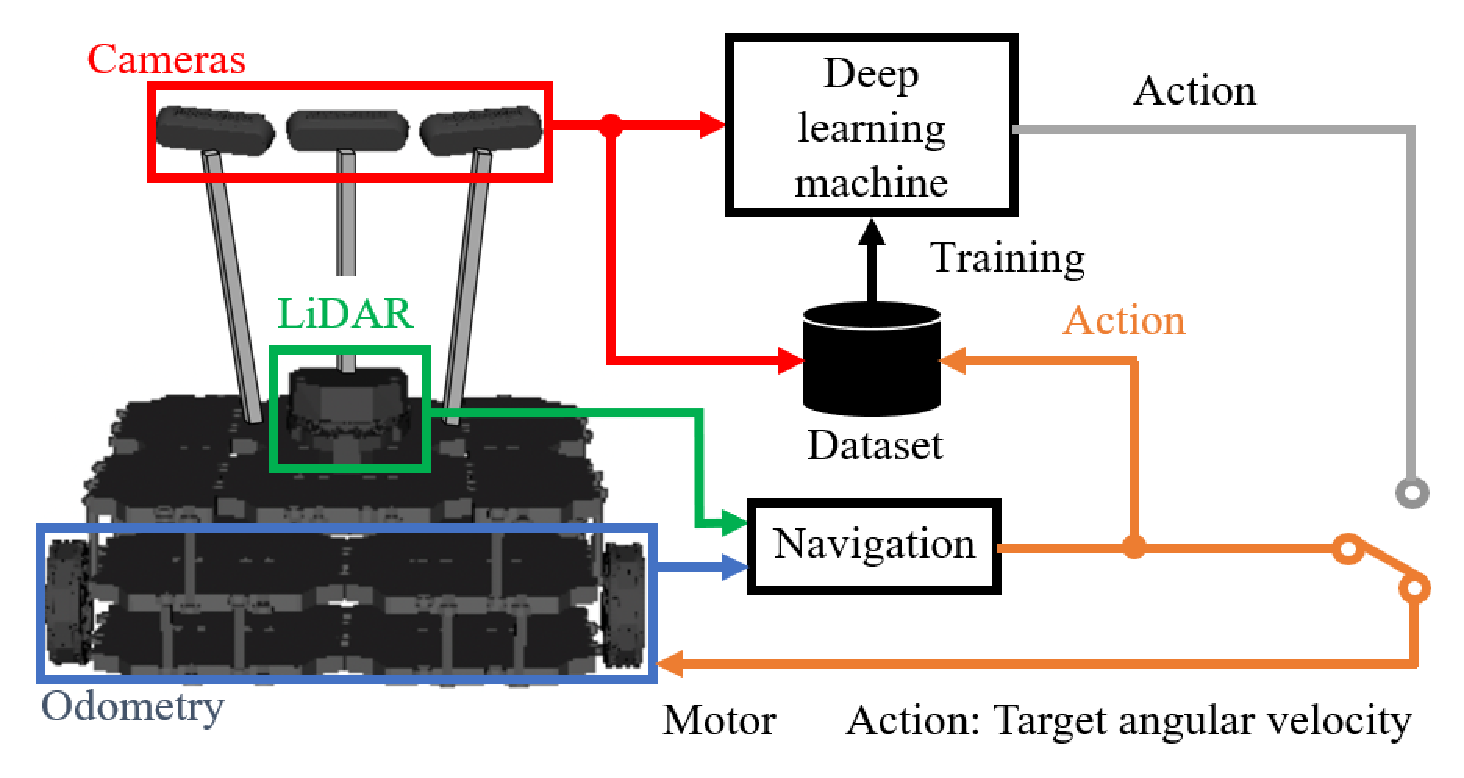
\includegraphics[keepaspectratio, scale=0.32]{fig/lm1.pdf}
    \subcaption{地図ベースの経路追従の模倣学習}
  \end{minipage}
  \begin{minipage}[t]{0.5\linewidth}
    \centering
    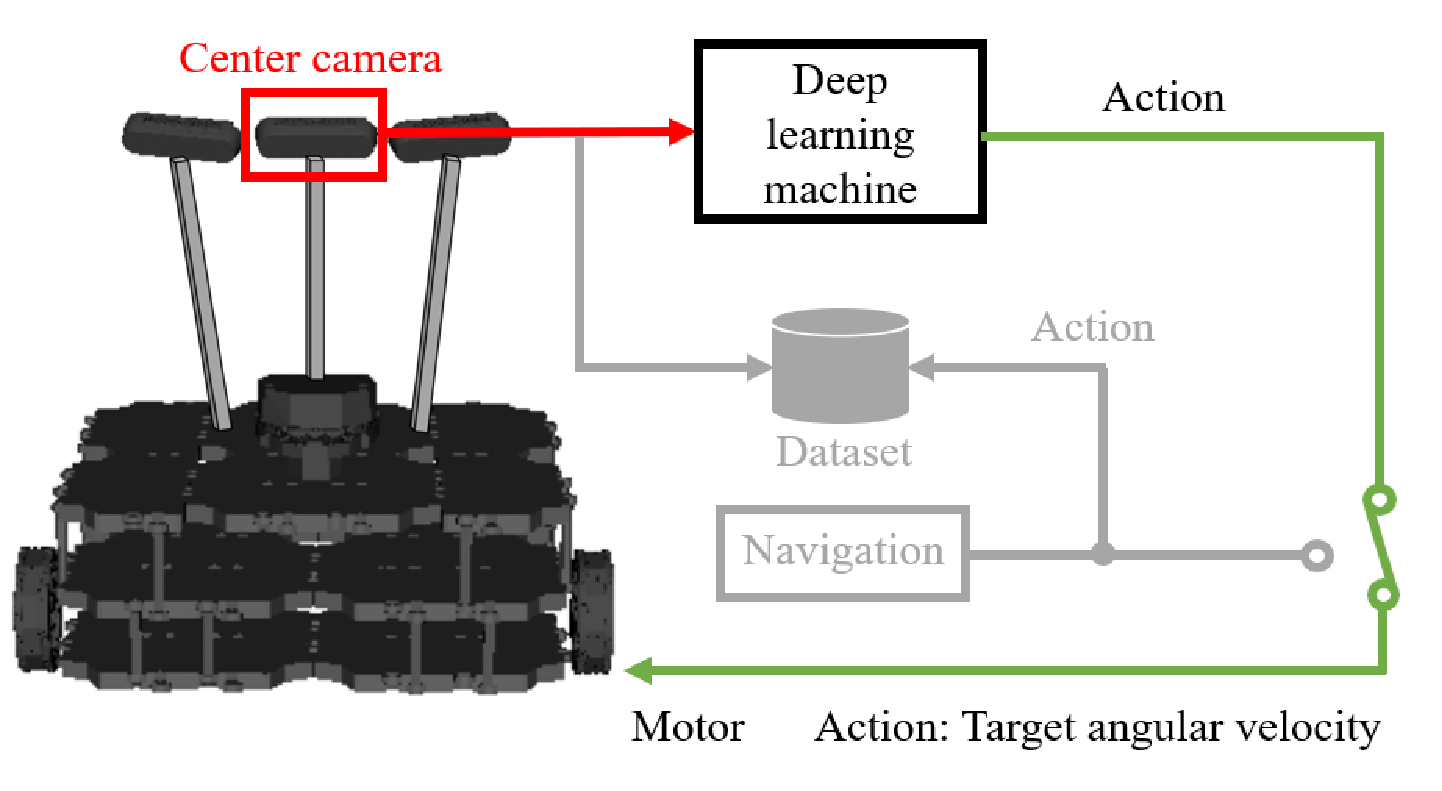
\includegraphics[keepaspectratio, scale=0.32]{fig/lm2.pdf}
    \subcaption{学習済みモデルを用いた視覚による経路追従}
  \end{minipage}\vspace*{2mm}
  \caption{模倣学習により視覚に基づき経路追従する手法}
\end{figure}




\section{研究計画}
日程を図ではるかなにかする


\section{入学後の抱負}
入学後は研究に尽力するのはもちろんのこと, 成果を上げ, 学会発表をする所存である.
また, 毎年本研究室で参加しているつくばチャレンジにおいて, 本研究の手法を用いて自律移動させ, 
完走することで新たな技術として回りに広げていきたい.技術交流として



\begin{thebibliography}{99}
  \small
  \bibitem{1}
  岡田眞也, 清岡優祐, 上田隆一, 林原靖男, “視覚と行動の end-
  to-end 学習により経路追従行動 をオンラインで模倣する手法
  の提案”, 計測自動制御学会 SI 部門講演会 SICE-SI2020 予稿
  集, pp.1148-1152, 2020.\\
  
  \bibitem{2}
  岡田眞也, 清岡優祐, 春山健太, 上田隆一, 林原靖男, “視覚と
  行動の end-to-end 学習により経路追従行動 をオンラインで
  模倣する手法の提案 -経路追従行動の修正のためにデータセッ
  トを動的に追加する手法の検討-”, 計測自動制御学会 SI 部門
  講演会 SICE-SI2021 予稿集, pp.1066-1080, 2021.\\
  
  \bibitem{3}
  W. Schwarting, J. Alonso-Mora, and D. Rus,
  “Planning and decision making for
  autonomous vehicles,” Annu. Rev, Vol. 1, No. 1, pp. 188-210, May 2018.\\
  
  \bibitem{4}
  U. Muller, J. Ben, E. Cosatto, B. Flepp, and Y. Cun, “Off-road obstacle avoidance
  through end-to-end learning,” Advances in neural information processing systems,
  Vol. 18, 2005.\\
  
  \bibitem{5}
  Bojarski, Mariusz, \textit{et al}.,
  “End to end learning for self-driving cars,” arXiv:1604.08316, 2016.\\

\end{thebibliography}



\end{document}
